\chapter{Team 4 Agent Design}\label{team_4_agent_design}

\section{Strategy Overview}
The overall agent strategy was determined by an evolutionary algorithm (see overview in \Cref{fig:evolutionOverview}) which allowed the agent to preemptively adapt to unknown environments. The evolutionary algorithm was further complemented by a trust score, which acted as a measure of the agent's perception of the trustworthiness of other agents in the tower. Additionally, the agent was given a cravings parameter which simulated how hunger would affect a human in the real world. This created a well-rounded agent that was able to dynamically adapt to the changing environment in order to survive. 

\begin{figure}[htb]
    \centering
    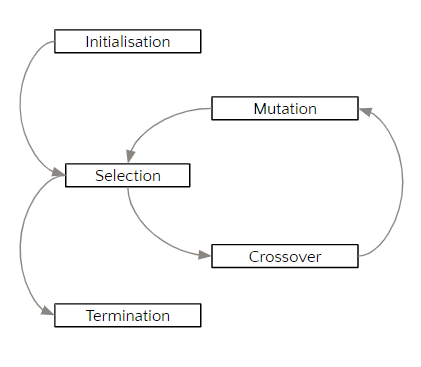
\includegraphics{006_team_4_agent_design/assets/evolution_overview.png}
    \caption{Overview of evolutionary algorithm.}
    \label{fig:evolutionOverview}
\end{figure}

\section{Evolutionary Algorithm}

In the fundamentals of evolutionary algorithms, every agent has a set of genes (or genotypes), which can express themselves (as phenotypes) in the way the agent interacts with its surroundings. Therefore, the aim is to find the optimal genotypes that will give phenotypes that are deemed to be favourable. This is implemented by seeing the performance of an agent according to a particular metric. This way the effect of each phenotype (and therefore underlying genotype) is put into perspective and ranked against the others. The most successful agents survive, while the less performant ones are killed off. When the surviving population reproduces, the resulting offspring will share the genes of both their parents, meaning they will have a mix of the most successful genotypes. Furthermore, there are some offspring with mutated genes and some that have identical genes to the previous generation for genetic variation. With this new population, the process is repeated to iteratively create more successful populations, as illustrated in \Cref{fig:team4evolve}.

\begin{figure}[htb]
    \centering
    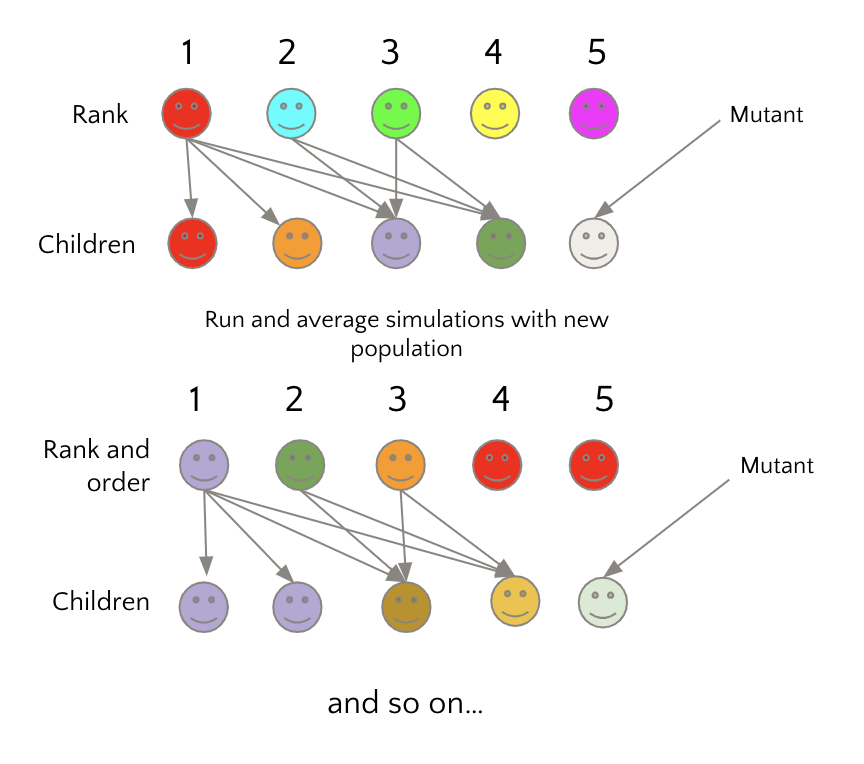
\includegraphics[width=0.7\textwidth]{006_team_4_agent_design/assets/evolve.png}
    \caption{Population selection process in an evolutionary algorithm.}
    \label{fig:team4evolve}
\end{figure}

Hence, with the use of an evolutionary algorithm, the final agent was the culmination of multiple generations of populations, with the genes of successful ancestors having been propagated and mixed. This meant it was a well-adapted agent which was robust to the many environments it could encounter in the tower. 

\subsection{Agent Genotypes}
To use evolutionary algorithms optimally, the genotypes that evolve should be well defined. This section outlines the two genotypes that were chosen as they were deemed to have the most effect on the survival of an agent in the system.

\subsubsection{FoodtoEat}\label{FoodtoEat}
\texttt{FoodToEat} was the amount of food the agent would eat on any given day of the simulation. Given the HP update curves in \Cref{updateHP}, it can be noted that any consumption past the threshold of 60 food had little to no effect on the HP gain of the agent. This meant that eating any more than that amount was wasteful and sub-optimal, so during the training process the algorithm was capped. This meant that the process could never learn to eat a value above 60, just as it could not learn to eat a value below 0.

\subsubsection{WaitProbability} \label{waitProbability}
\texttt{WaitProbability} was the probability that the agent would not eat on any given day of the simulation. This is a probabilistic way of creating the agent, which is ideal to replicate the unpredictability of the real world. Having other implementations such as a hard-coded number of days to wait would give a much more robotic and predictable agent. This was especially apparent when initialising homogeneous populations of the evolutionary agent in the tower since they would all wait and eat at exactly the same times. With the probabilistic approach, this is not the case, and there was still a way for the agent to express a wanting to abstain from eating food on a particular day.

\subsection{Health Levels}
In order for these genotypes to be viable in the learning process, the values they could take had to be limited. The \texttt{FoodToEat} and \texttt{WaitProbability} were inherently limited to lie between 0-60 and 0-100 respectively, but there were many conditions under which the agent would have to choose between these values. It was decided that the agent's HP was the most apt factor in its decision making process. Hence, the agent's HP was divided up into different bands as a means of classifying the agent's current health into broader categories. The division resulted in four levels being created: Critical, Weak, Healthy and Strong with the range of HP corresponding to each level displayed in \Cref{tab:healthLevels}.

\begin{table}[htb]
    \centering
    \begin{tabular}{| c | c |}
    \hline
    Health Level & HP Range \\
    \hline
    \hline
     Critical & 3-9 \\ 
    \hline
     Weak &  10-39\\  
     \hline
     Healthy &  40-69\\
     \hline
     Strong & 70-100 \\
     \hline
    \end{tabular}
    \caption{Overview of the different health levels and their corresponding HP ranges.}
    \label{tab:healthLevels}
\end{table}

In each health band, the agent would consume a certain amount of food with a given probability of waiting before eating. The division of HP into broader bands reduced the complexity of the learning process greatly as compared to when optimising food intake for every possible HP value, and was therefore chosen as a good compromise.

\subsection{Cravings}

To implement a more realistic and life-like element to the agent, a cravings trait was added. The cravings of the agent would be increased as the desire for food increases and decreased otherwise.

Cravings directly effected the \texttt{waitProbabilities} put forward in \Cref{waitProbability}. As days pass without seeing food on the platform, the agent's craving increases, and in turn, its probability of waiting to eat decreases. The intuition behind this was that as more days pass without seeing food, the agent should eat when it can as there may not be many opportunities to do so in the future and may potentially lead to death.\newline

An agent's craving was altered in a few different scenarios:
\begin{enumerate}
    \item Food not seen on the platform - If the agent has not seen food in $x$ days, cravings is increased by $x$. Otherwise, the craving is decreased by two for everyday food is seen on the platform. 
    \item Eating food - When the agent eats food, craving is decreased proportionally to the amount of food the agent has eaten \emph{i.e.} $cravings = cravings \left(1 - \frac{foodeaten}{desiredfood}\right)$
\end{enumerate}

This enabled the agent to perform house-keeping as it reduced the likelihood of a scenario where the agent does not eat for long periods of time, preventing self-inflicted damage as a result of \texttt{waitProbability}. 

It should be noted that the training process did not learn the values to assume in the critical region. These values were instead hard-coded as the agents `survival instinct', whereby it ate what it needed to leave critical health. This added a component of self-healing to the agent.

\subsection{Agent Performance Metrics}
\begin{table}[hbt]
    \small  
    \centering
    \resizebox{\textwidth}{!}{%
    \begin{tabular}{| m{5em} | m{13em} | m{14em} |}
    \hline
    Averaging method & Advantages & Disadvantages  \\
    \hline
    \hline
        Global Lifespan & 
        -- Attempted to maximise lifespan of all agents including itself 
        
        -- Struck a balance between self preservation and global welfare. 
        & 
        -- Didn't reach optimum strategy with no deaths
        
        -- Agent had little effect on global lifespan. \\
        \hline
        Team Four Agent Lifespan & 
        -- Maximised agent 4 survival (attempted to satisfy itself)
        
        -- Actions of others had less effect on survival of agent. 
        & 
        --  Disregarded other agents in the tower
        
        -- Failed to create stable system as all food was consumed by agent. \\
        \hline
        Other Agent Lifespan & 
        -- Attempted to reach optimum state of co-operation
             
        -- Worked for the betterment of society (for the satisficing of each agent).
        &
        -- Put itself at risk while eating minimal amount of food
             
        -- Agent had little effect on global lifespan. \\
        \hline
    \end{tabular}}
    \caption{Pros and cons of different averaging methods chosen for agent parameter optimisation.}
    \label{tab:lifespanAveraging}
\end{table}

When training the agent, there were multiple ways to interpret any given metric. For this project, it was decided that the metric that gave the most accurate depiction of agent fitness was their lifespans. For this reason, average lifespans were used during the training process, but even so, there were many options for how to take these averages. The pros and cons of our chosen averaging methods are given in \Cref{tab:lifespanAveraging}.

The agent was trained to determine three personalities: selfish, neutral and selfless. The selfish nature of the agent was designed for self-prioritisation over community welfare. The selfless configuration was trained to optimise the global life expectancy whereby the agent would try to reduce global deaths per iteration. The neutral configuration aimed to strike a balance between the two previous configurations, trying to optimise overall life expectancy, inclusive of itself. Through this method, the agent has the capabilities to maximise its utility at the micro level and sustainability at the macro level.

\section{Message Passing}
To create an agent that can self-organise according to its neighbours, communication was vital so that its actions would vary according to a changing environment. Both message passing, and treaties had been implemented to account for the many possible situations that could affect the agent. 

\subsection{Simple Messages} \label{team4SimpleMessages}
For simple communication, the agent was able to both send messages and handle the messages received from other agents.

\subsubsection{Handling Message Generation}
There were two scenarios the agent considered when determining what message it would want to send. The first was when the agent’s health status had reached critical. A message was sent to the floor above requesting them to leave just enough food for the agent to survive. Messages were also sent so that the agent could learn about the amount of food another agent (on a different floor) intended to take, as well as the amount of HP they had. Not all recipients would respond to these requests, so to maximise the agent’s interaction and learning, it yelled across multiple floors, both above and below.

\subsubsection{Handling Received Messages}
Many other agents from multiple floors were likely to send their own requests, so various handler functions were implemented to determine the preferred response. When a message was first received, it was stored into one of two memory buffers. One for recording messages requesting a particular amount of food to be left, and another for other message types. Since the agent could only respond to one message per tick in the simulation, it prioritised those asking for food to be left first. To determine if the agent should accept the request, it waited for the platform to reach its own floor. It then compared if the available amount on the platform after the agent ate was greater or equal to the amount being requested. If this was true, it left that amount and sent a response saying yes. For all other message types, the agent replied honestly to a given query. 

\subsection{Treaties} \label{team4Treaties}
The agent accepted any subset of treaties that were in line with its own goals. The first few conditions were all dependent on the availableFood. In the case that the agent was within a threshold of the critical region (this being the critical health level multiplied by 2), the corresponding treaty was rejected. The agent also rejected any treaties where the condition was dependent on having available food less than a certain amount. Finally, all treaties requiring the agent to leave food less than the critical amount were rejected, so as to afford agents on lower levels of the tower the opportunity to survive if they were in critical condition. 

Similarly, treaties were also subject to the condition of HP. The agent rejected all treaties where the conditional HP was less than the critical band. Here, the agent would be at the point of desperation and should not be forced into any action. Additionally, treaties may have been requested where the condition of the agent was required to be less than a certain HP, or the agent was required to be placed on a higher floor number. These would lead to a significant disadvantage for the agent as treaties are binding. Consequently, treaties with these conditions were all rejected. When the duration was greater than the maximum number of days in critical, it could lock the agent into a forced action resulting in its death. To ensure this didn't happen, the agent rejected all such opportunities. 

The agent also propagated accepted treaties, giving other agents the option to follow a similar ideology to its own. The agent could then enforce it's influence on the social order within the chaos of the tower. On the other hand, treaties that were not accepted were not further propagated. This was because the agent did not want to spread methods that were in detriment to it's own as this would pose a risk to the social order enforced by the agent itself.

\section{Trust Score}
The trust score was a parameter that allowed a more dynamic approach to be built on top of the relatively static evolutionary algorithm. The agent used this trust score to build a global trust network based on its local interactions using the message passing and treaty-based techniques mentioned in \Cref{team4SimpleMessages} and \Cref{team4Treaties}. The trust score allowed the agent to alternate between the three personalities: selfless, neutral and selfish. \Cref{fig:team4updateHP} shows examples of certain trust score updates where the agent was able to vary its own configurations after altering its trust score parameter. This gave the agent an element of self-optimisation as it was allowed to adapt to information gained from its environment and other local interactions. 

\begin{figure}[htb]%
    \centering
    \subfloat[\centering Decrease in trust]{{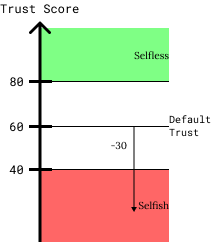
\includegraphics[width=0.3\linewidth]{006_team_4_agent_design/assets/selfish.png}}}%
    \qquad
    \subfloat[\centering Increase in trust]{{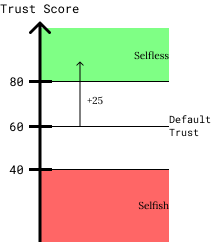
\includegraphics[width=0.3\linewidth]{006_team_4_agent_design/assets/selfless.png}}}%
    \caption{Change in agent configuration as a result of global trust score.}%
    \label{fig:team4updateHP}%
\end{figure}

Trust score for an agent was increased through a multitude of interactions. As the system was designed to be honest, the agent increased trust score when the floor above took a certain amount of food that was deemed to be an acceptable value (less than the maximum food taken in the selfish configuration) and communicated this to the agent. Additionally, when the floor below left a certain amount of food, the agent also increased its trust score.

In the cases where the floor above left a certain amount of food and the agent below also took a certain amount of food, the agent did not instantaneously increase the trust score. Instead, the agent verified that the agents above and below followed through with the actions mentioned through the \texttt{verifyResponses} function. The agent used the function once it received replies to \texttt{RequestLeaveFood} and \texttt{RequestTakeFood} messages. Whenever a message was sent, it was stored by the agent. This allowed the agent to correspond replies and responses to the appropriate sent messages. All responses which were not in accordance with the agent's ideology, or were not replied to at all, were sanctioned through a decrease in the global trust score metric. A decrease in trust score led the agent to act more selfishly, which acted to the detriment of other agents. This meant that there was some form of punishment for antisocial behaviour from other agents to stop them destroying the social order constructed by the agent within the tower.

In the case of the agent on the above floor leaving food, the agent first checked whether the platform was on its current floor through the function \texttt{PlatformOnFloor}. The global trust score was then updated through the function \texttt{updateGlobalTrustLeaveFood}. The agent used the function \texttt{CurrPlatFood} to check the food on the platform and verify that the food on the platform was greater than or equal to the food that the agent on the above floor had said they were going to leave. This resulted in an increase in the trust score. In the case where an agent lied (though this should not be possible in simulation), the agent reduced its trust score as a consequence of lying. 

In the case of the agent below taking food, the agent always stored the food left on the platform after they had eaten. When a response to a \texttt{RequestTakeFood} message was received from the below floor, the agent first checked whether the below agent had eaten through the function \texttt{neighbourFoodEaten}. As the food left on the platform was stored by the agent and the agent being able to see the food on the below platform through the function \texttt{CurrPlatFood}, the agent was able to verify that the agent below had been truthful. This was done by adding the food that the agent had supposedly taken to the food that was currently on the platform and verifying it against the food that had left this agent's platform.

The agent updated the trust score based on the messages sent and received to and from other agents. This showcased self optimisation, since the agent chose a configuration to follow based on interactions with others and observation of their actions. The agent then used this trust score as an indicator of when to switch between the three different personalities. With high trust, the agent was inclined to be more selfless, and with low trust the agent was likely to be more selfish.

In the case, where an agent did not respond to our sent messages, the trust score is decreased overall. This allowed the agent to be empowered in its action through logical reasoning as the agent was able to enforce a more selfish personality due to miscommunication. This further warranted our agent to sanction members within the local environment when they responded negatively to the agent's overall ideology of trying to create a selfless utopia. These actions allowed the agent to idealise Ostrom's fifth principle of sanctioning further as miscommunication is punished as it is deemed to be a necessity in the collaborative multi-agent system that the agent tries to create.

\begin{figure}[htb]
    \centering
    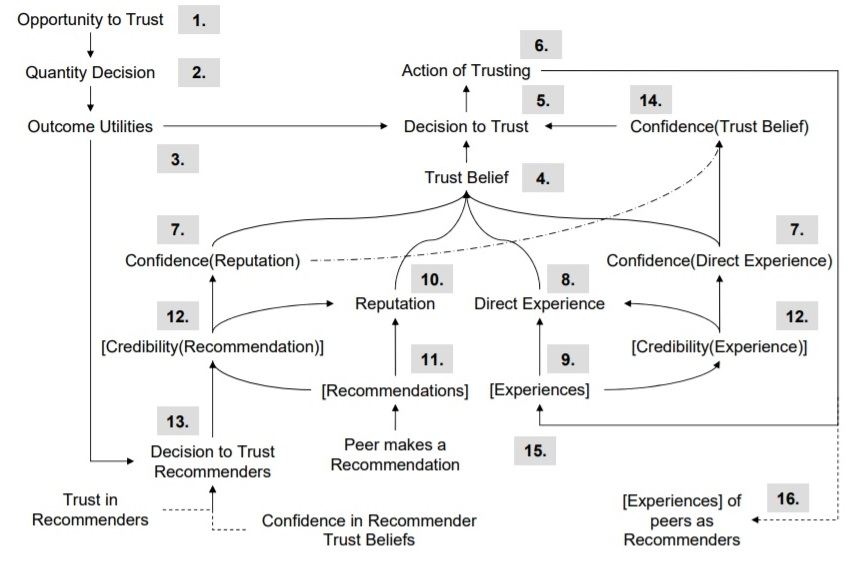
\includegraphics[width=0.85\textwidth]{006_team_4_agent_design/assets/JeremyPittTrustFramework.jpg}
    \caption{An illustration showing the formal model of the Trust Framework. \cite{JeremyPittSlides}}
    \label{fig:TrustFramework}
\end{figure}

The trust score acted as an element of symbiosis between the learning-based evolutionary algorithm that the agent was originally employed with and a self-organising strategy. Additionally, it allowed the agent to improve on it's relatively static structure to become more dynamic so as to adapt to the changes in it's surrounding environment. This was advantageous as the agent was able to use its pre-defined metrics in tandem with trust score and cravings to adapt within the tower depending on its social construction of reality. The trust score enacted the formal model (as shown in \Cref{fig:TrustFramework}) of a trust framework whereby the opportunity to trust is employed through communication and action, whilst the quantity decision is made through every individual agent strategy. Through local trust based modelling of a global trust score, the agent is able to implement the outcome utilities portion of the trust framework.

\section{Experimentation and Results}

\subsection{Baseline Comparisons}
In order to evaluate the performance of the agent, it was compared to two baselines - the default agent and the random agent. The time taken for the system to stabilise (\emph{i.e.,} time taken for the agents to organise into a structure that led to no future deaths) into a viable social order was measured. Tests with homogeneous populations of Team 4 agents, default agents and random agents were conducted, which highlighted that the two baselines never stabilised, whilst the Team 4 agent did. This was evident from \Cref{fig:baselinecomps} which showed the number of deaths for the Team 4 agents eventually stagnating however, this did not occur for the other two agent types. This was because the agent was able to build a trustworthy local perception which resulted in a positive outlook of the environment, allowing all agents to tend towards selflessness. This selfless behaviour enacted utilitarianism as the agents were able to maximise the average food left on the platform after a day had passed, ensuring that there was no wastefulness, whilst the overall population was still able to survive. 

\begin{figure}[htb]%
    \centering
    \subfloat[\centering Random Agent ]{{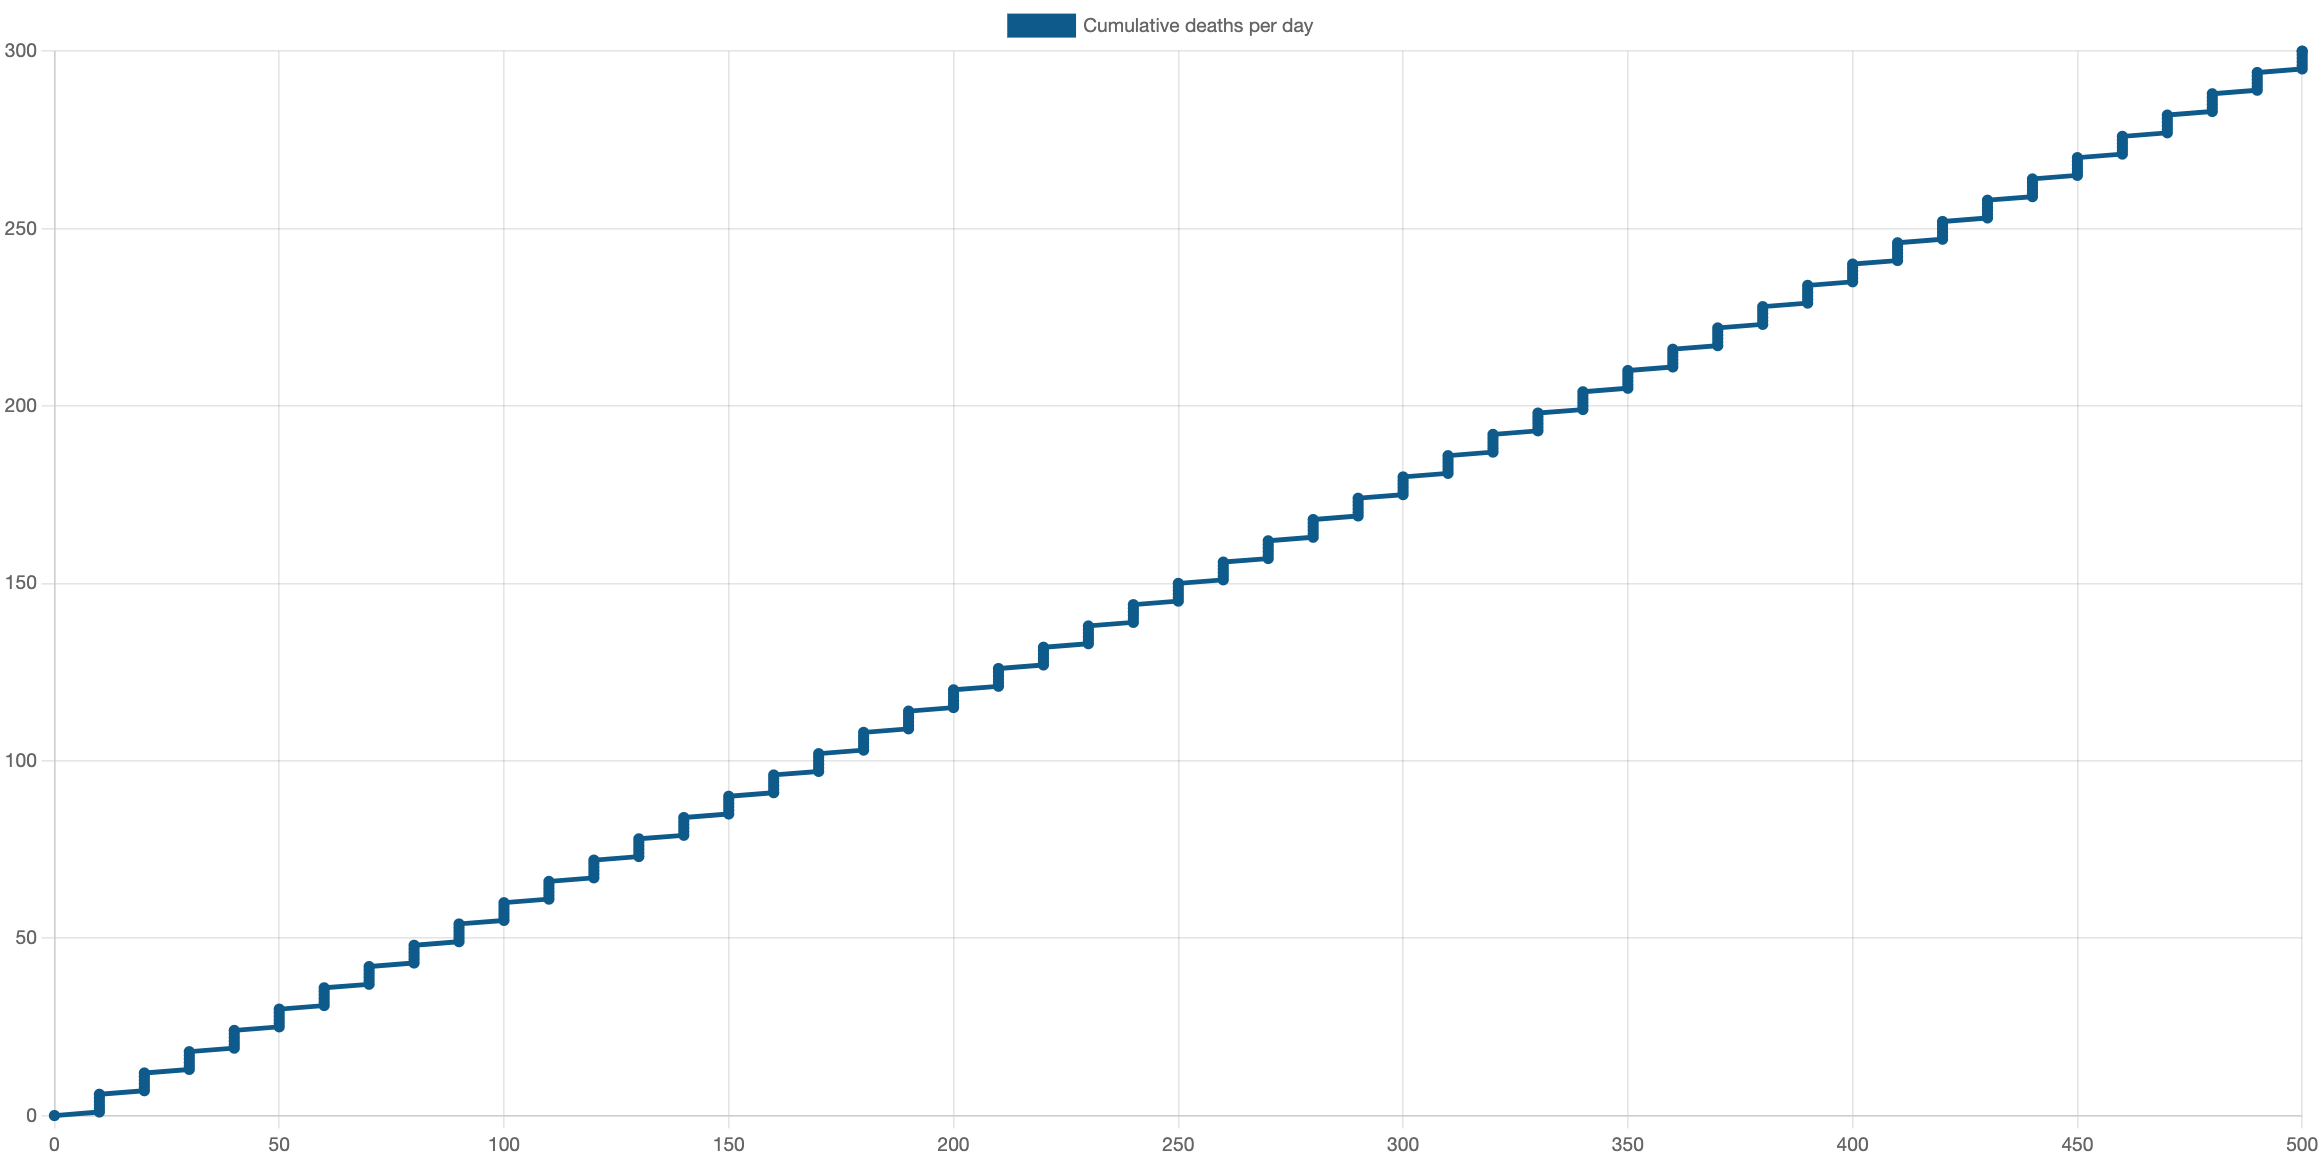
\includegraphics[width=0.4\linewidth]{006_team_4_agent_design/assets/unstabledefault.png}}}%
    \qquad
    \subfloat[\centering Default Agent ]{{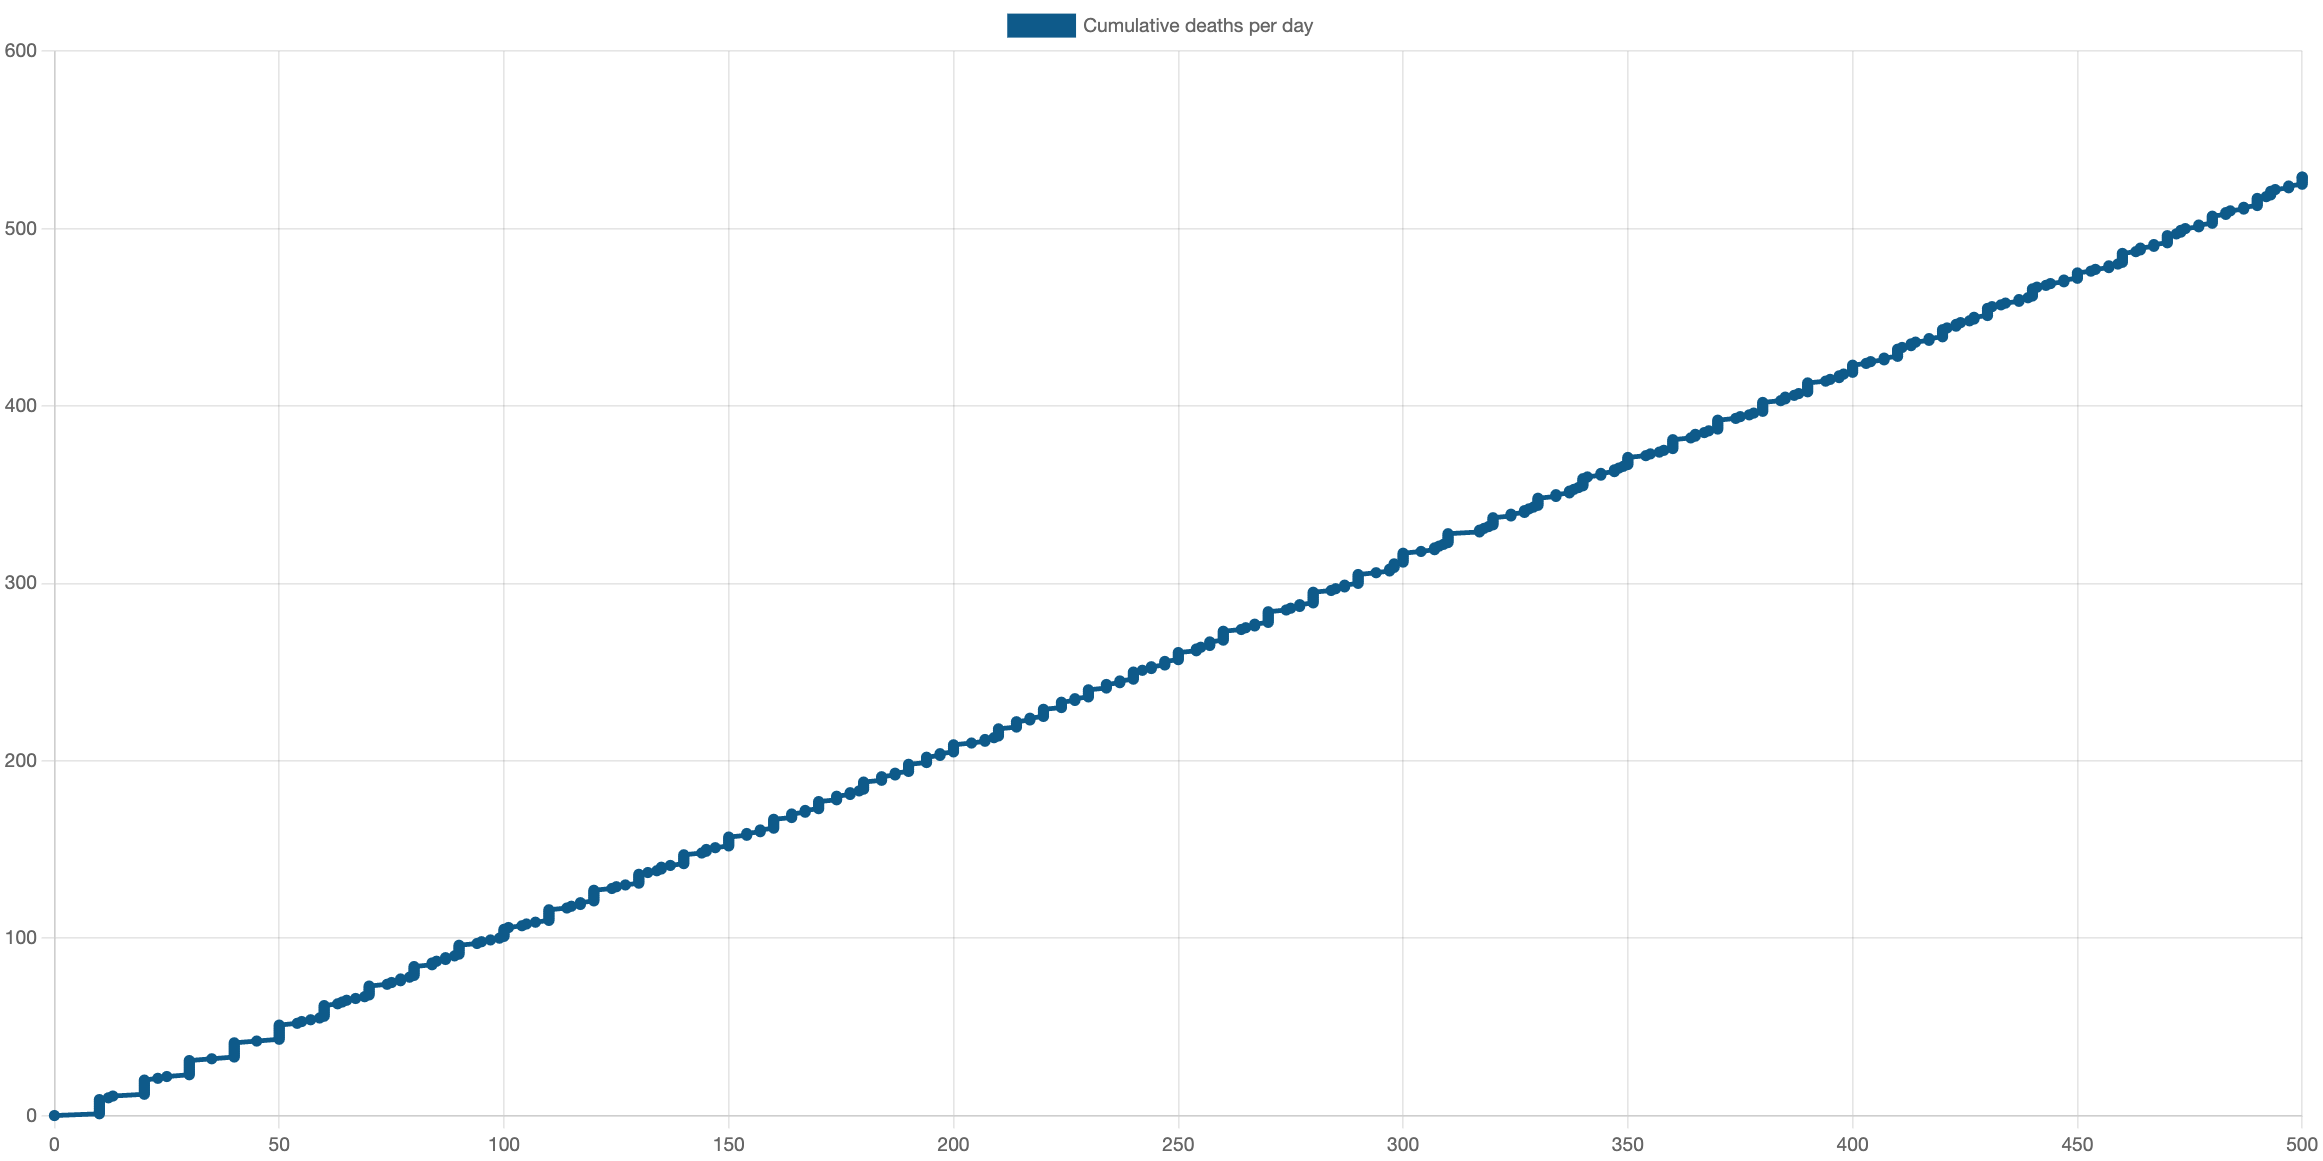
\includegraphics[width=0.4\linewidth]{006_team_4_agent_design/assets/unstablerandom.png}}}%
    \qquad
    \subfloat[\centering Team 4 Agent]{{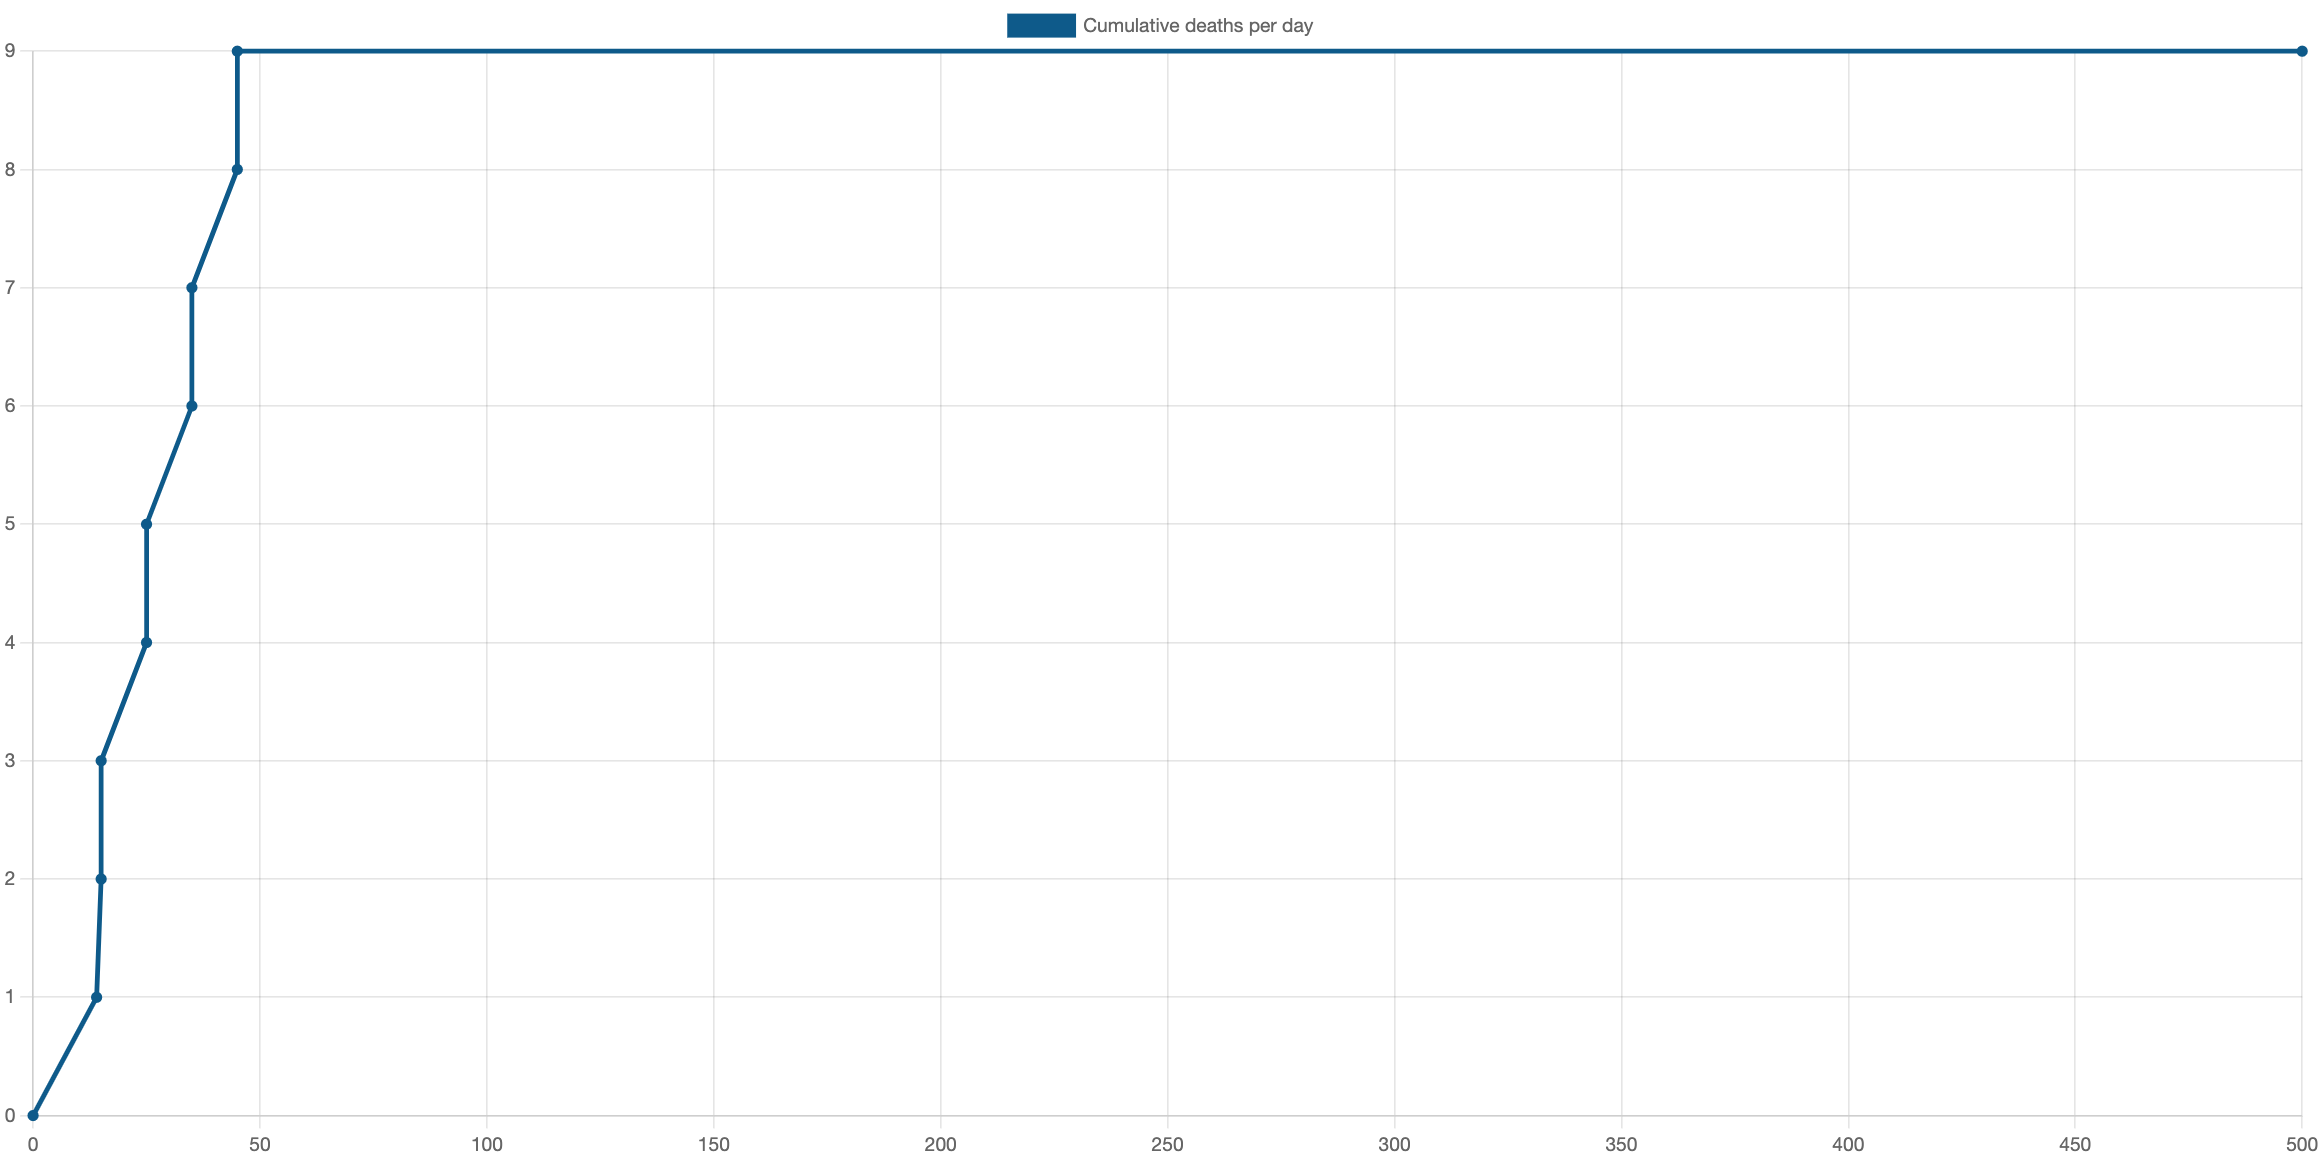
\includegraphics[width=0.4\linewidth]{006_team_4_agent_design/assets/stableus.png}}}%
    \caption{Graphs showing stabilisation times for various homogeneous populations of agents in the tower.}%
    \label{fig:baselinecomps}%
\end{figure}

\subsection{Stabilisation Times}

\subsubsection{Effect of Reshuffle Period}
\Cref{tab:reshuffleStabilisationTimes} shows the time taken for a system to stabilise with different numbers of reshuffle days. With longer reshuffle days, it took longer to stabilise as there were fewer opportunities for the agents to communicate with one another. This was the case since communications only occurred with a limited number of floors above and below the agent resulting in the agent only being able to create a limited view of its environment without reshuffling. 

\begin{table}[htb]
    \centering
    \begin{tabular}{|c|c|c|}
    \hline
    Reshuffle Days & Deaths & Days to Stabilise\\
        \hline
        \hline
        7 & 0 & 0 \\
        \hline
        25 & 4 & 24 \\
        \hline
        50 & 10 & 58 \\
        \hline
        100 & 18 & 94 \\
        \hline
    \end{tabular}
    \caption{Table showing stabilisation time for various reshuffle periods with 16 Team 4 agents.}
    \label{tab:reshuffleStabilisationTimes}
\end{table}

\subsubsection{Effect of Food Scarcity}
\Cref{tab:scarcityStabilisationTimes} shows the time taken for a system to stabilise with different levels of food scarcity. This scarcity was measured in amount of food per agent, meaning this value could decrease with both the food on the platform or number of agents in the tower. With more scarcity, the system took longer to stabilise since food became a more sought after resource, resulting in more conflict through competition over the shared resource which requires a longer time period for dispute resolution. When there was total scarcity of food, the system did not stabilise which was expected because there was simply not enough food for the agents to survive. With total abundance, the agents never die and form a stable system from the very beginning.

\begin{table}[htb]
    \centering
    \begin{tabular}{|c|c|c|}
    \hline
    Food Scarcity (food per agent) & Deaths & Days To Stabilise  \\
        \hline
        \hline
        Total Scarcity ($<$3) & $>$402 & does not stabilise \\
        \hline
        Satisfice (=3) & 27 & 167 \\
        \hline
        Total Abundance ($>$5) & 0 & 0 \\
        \hline
    \end{tabular}
    \caption{Table showing stabilisation time for various levels of food scarcity, reshuffling every 25 days, 500 days in total.}
    \label{tab:scarcityStabilisationTimes}
\end{table}

\subsubsection{Effect of Random and Selfish Agents}

A random agent was defined as an agent that eats random amounts of food on any given day. A selfish agent was defined as an agent that eats the amount of food it needs to remain at full HP. It was interesting to note the effect of each agent on homogeneous populations of Team 4 agents, and how many of them it took to destabilise the system.

\Cref{fig:selfishagentcomps} and \Cref{fig:randomagentcomps} show the behaviour of Team 4 agents with selfish and random agents respectively. In both instances, a similar trend was noticed; there were periods of stability but the system was disrupted to an unstable state soon after. Instances with the random agent were explained by the fact that it could not communicate with other agents and therefore no meaningful relationships could be created. Hence, even if stability was achieved through the communication between Team 4 agents, the unpredictable behaviour of the random agent quickly disrupted this. 
\newline
With the selfish agent, despite communication being present, Team 4 agents became selfish themselves due to distrust and a lack of communication from selfish parties. This meant both agent types acted in their own self interests causing the system to destabilise and the number of deaths increase.

\begin{figure}[htb]%
    \centering
    \subfloat[\centering 8 Team 4 agents with one selfish agent ]{{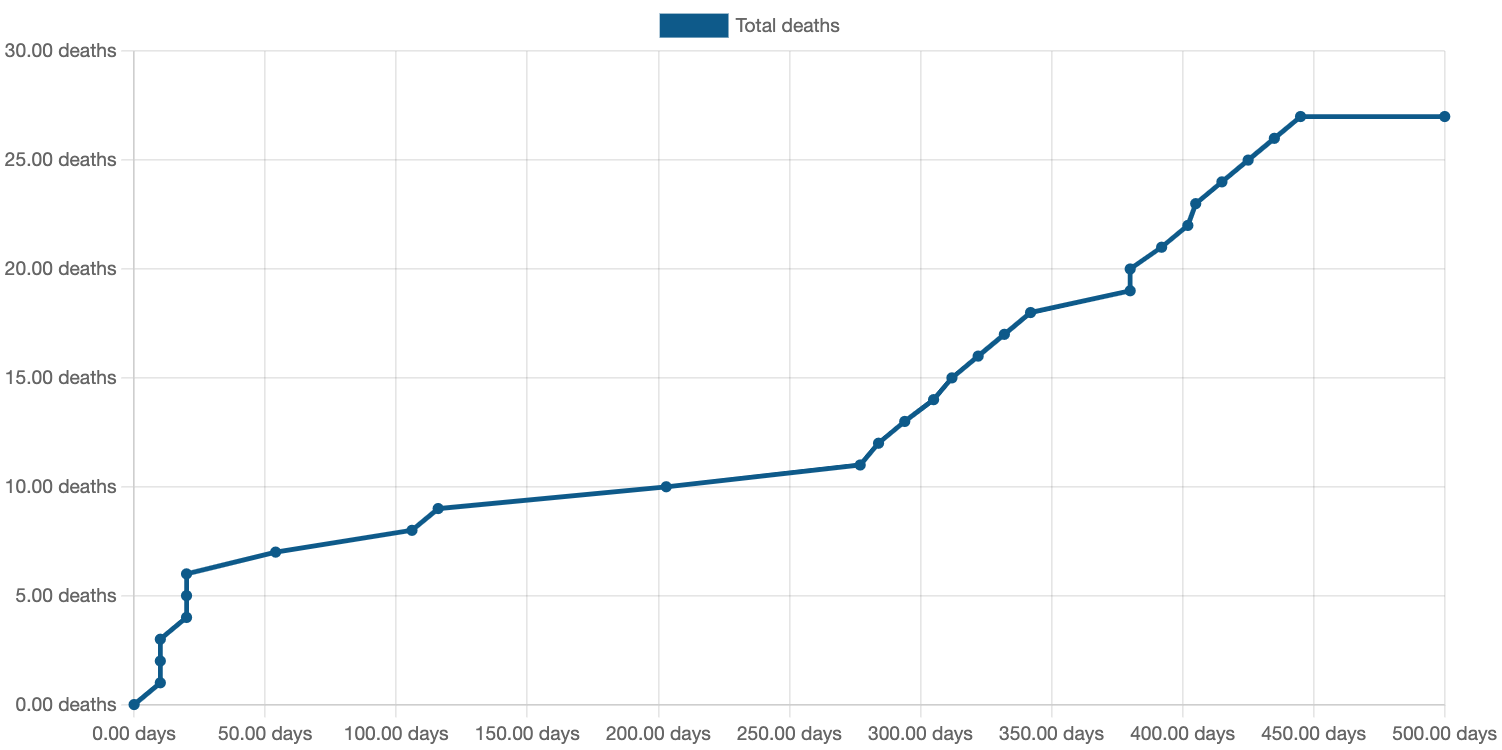
\includegraphics[width=0.45\linewidth]{006_team_4_agent_design/assets/selfishRuns/oneOtherSelfish.png}}}%
    \qquad
    \subfloat[\centering 8 Team 4 agents with two selfish agents ]{{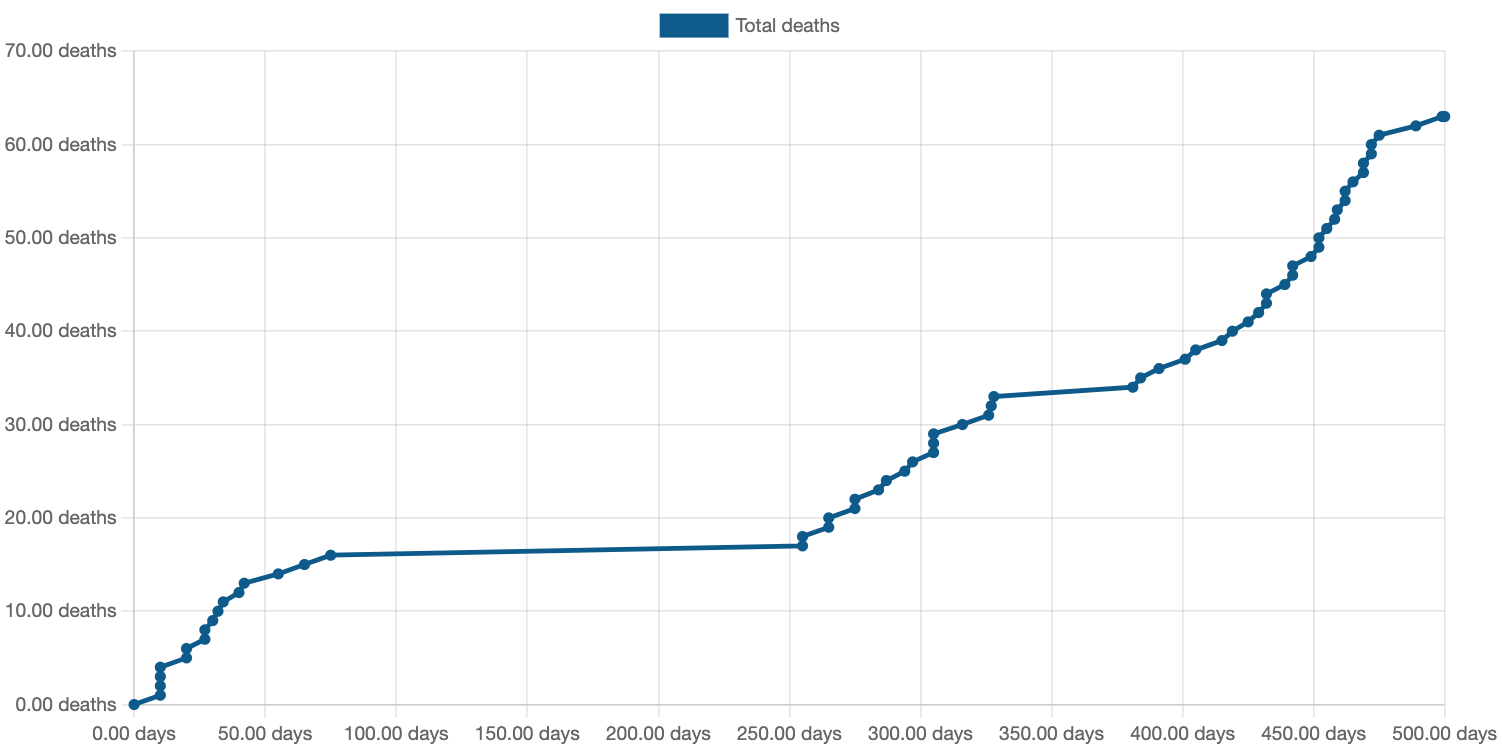
\includegraphics[width=0.45\linewidth]{006_team_4_agent_design/assets/selfishRuns/twoOtherSelfish.png}}}%
    \caption{Impact of selfish agents on system stability}%
    \label{fig:selfishagentcomps}%
\end{figure}

\begin{figure}[htb]%
    \centering
    \subfloat[\centering 8 Team 4 agents with one random agent ]{{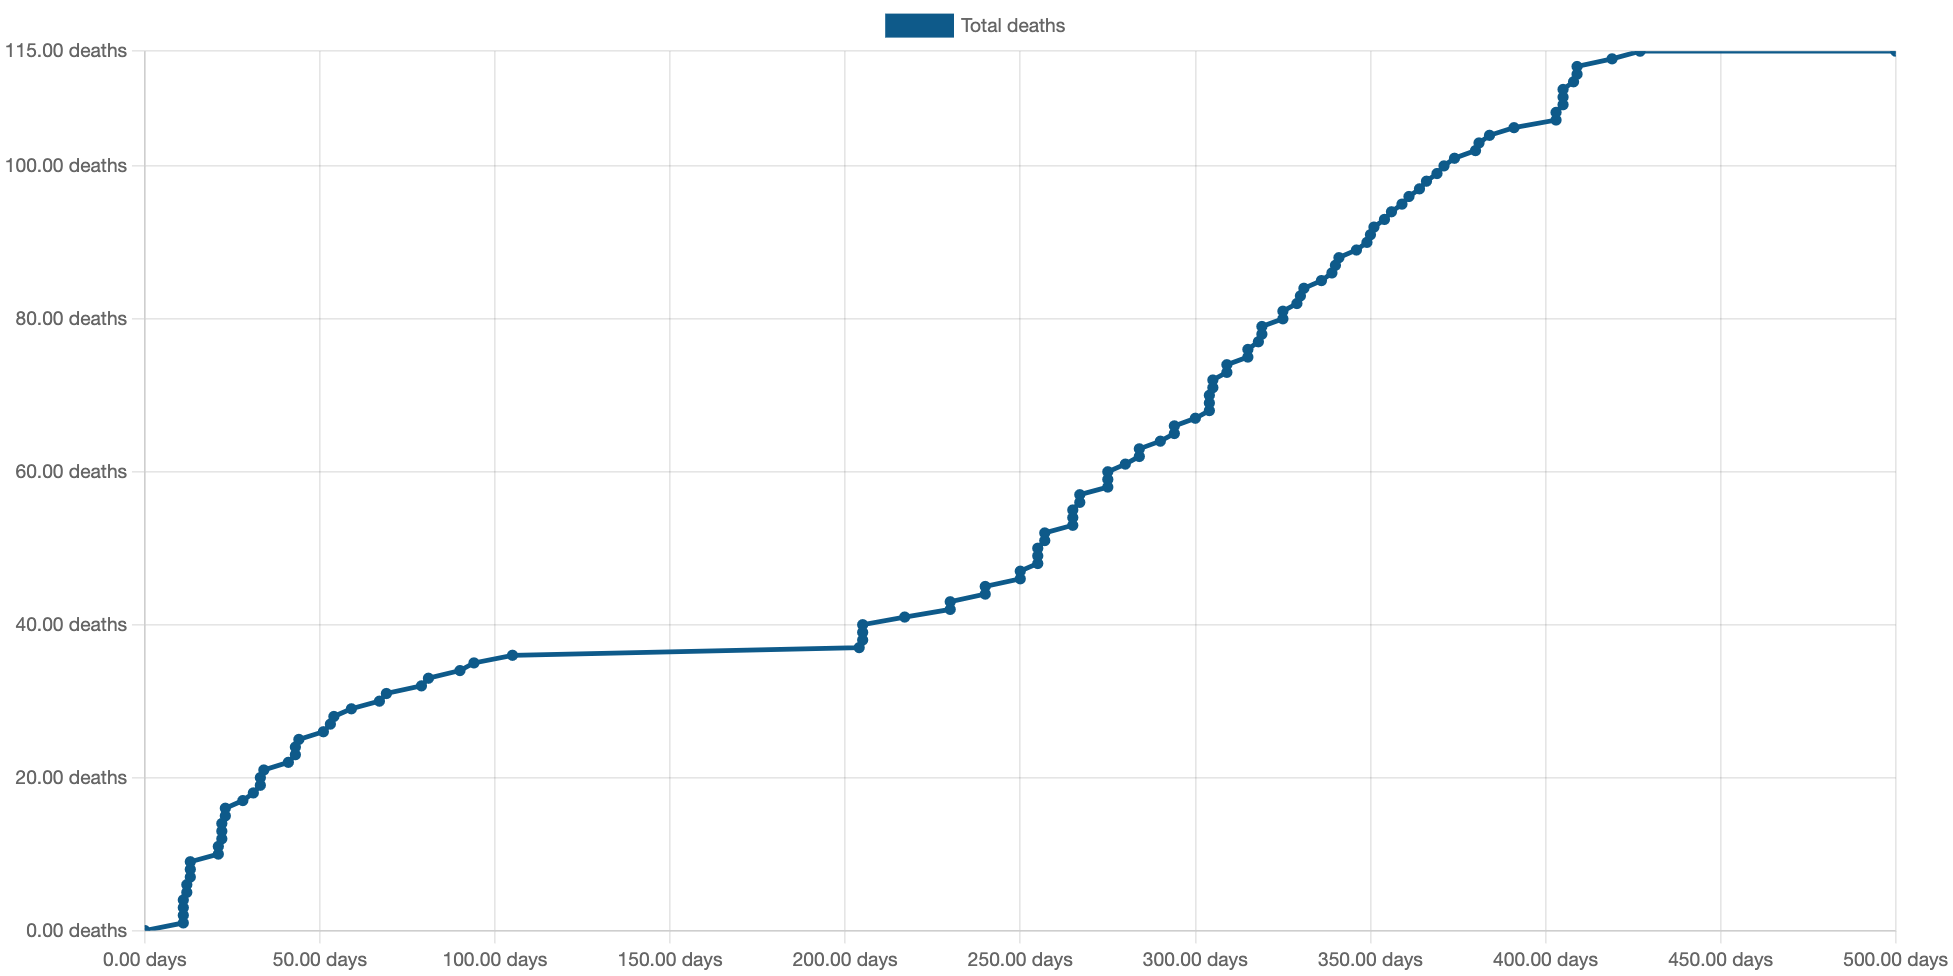
\includegraphics[width=0.45\linewidth]{006_team_4_agent_design/assets/randomRuns/oneOtherRandom.png}}}%
    \qquad
    \subfloat[\centering 8 Team 4 agents with two random agents ]{{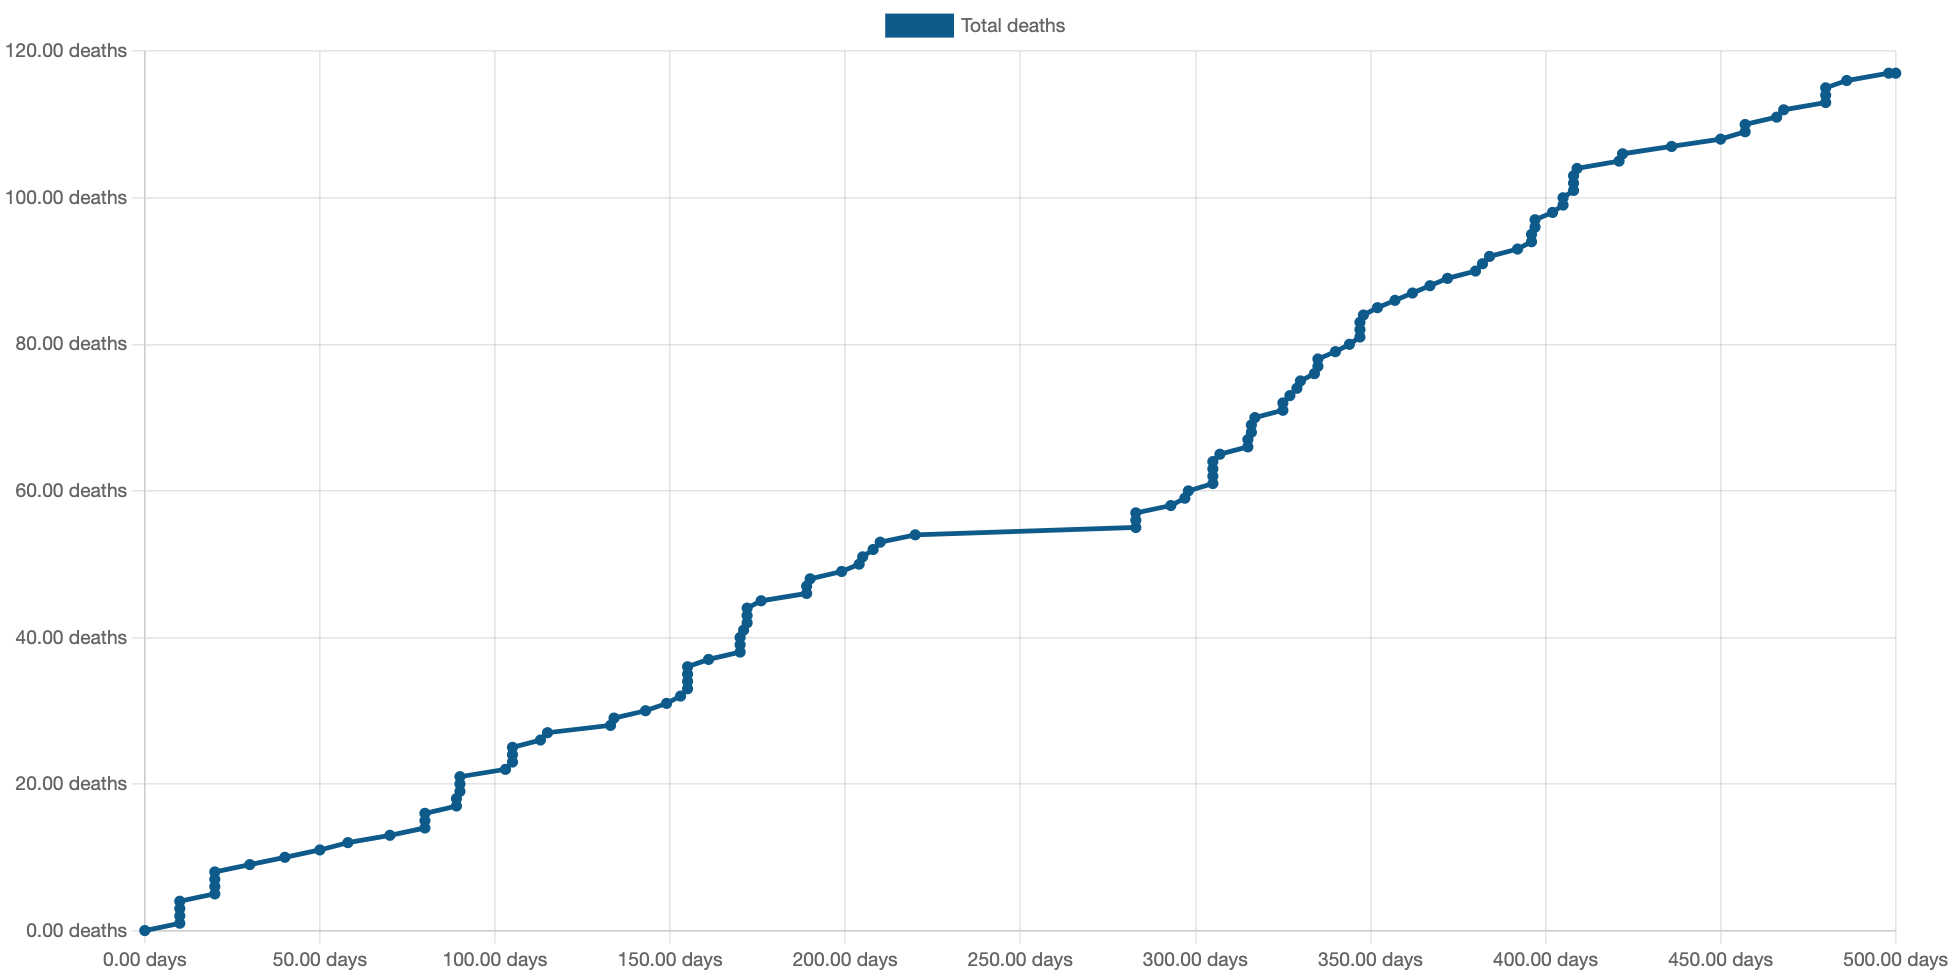
\includegraphics[width=0.45\linewidth]{006_team_4_agent_design/assets/randomRuns/twoOtherRandom.png}}}%
    \caption{Impact of random agents on system stability.}%
    \label{fig:randomagentcomps}%
\end{figure}

Overall, it can be said that the strategy of our evolutionary agent was very fragile and was easily effected by other more disruptive strategies.

\subsection{Communications and Interactions}

\subsubsection{Overview of Communications}
\Cref{fig:commsChart} shows the communications between agents in the tower on a particular run. A variety of messages were passed around, with the colours representing a particular message type. Theoretically, if the evolutionary agent had meaningful communications with other cultures, it should have been able to coexist with them.

\begin{figure}[htb]
    \centering
    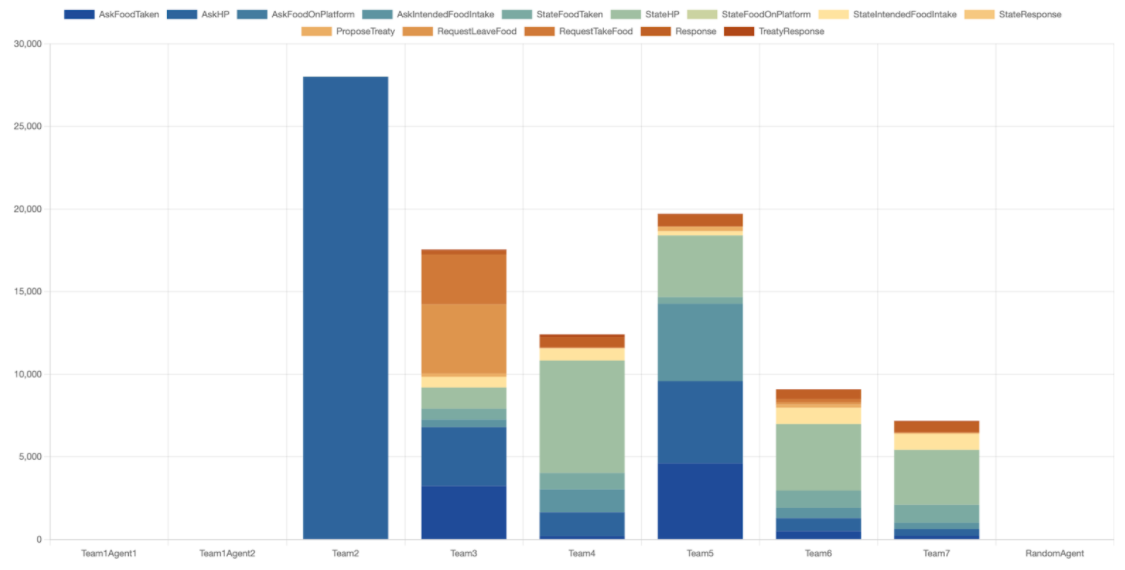
\includegraphics[width=0.85\textwidth]{006_team_4_agent_design/assets/communications_chart.png}
    \caption{A bar graph illustrating the various communications between agents.}
    \label{fig:commsChart}
\end{figure}

\subsubsection{Subsequent Compatibility with Other Cultures}
\Cref{tab:agentCompatibility} shows the compatibility of the evolutionary agent culture compared to the various cultures of other implemented agents. It is clear Teams 3, 5 and 7 were very compatible with the evolutionary agent as a result of fair communication allowing the agents to form a viable social structure, resulting in 0 deaths after a certain period of time. Teams 5 and 7 were particularly fast in forming this structure, suggesting that communication between the two were very efficient.

\begin{table}[htb]
    \centering
    \begin{tabular}{|p{5em}|p{5em}|p{5em}|p{5em}|p{9em}|}
    \hline
        Other Agent Team & Number of Deaths & Our Deaths & Other Deaths & Compatible? (stabilises within 500 days) \\
         \hline
         \hline
        2 & 222 & 146 & 76 & No \\
         \hline
        3 & 82 & 59 & 23 & Yes \\
         \hline
        5 & 2 & 1 & 1 & Yes \\
         \hline
        6 & 259 & 161 & 98 & No \\
         \hline
        7 & 4 & 0 & 4 & Yes \\
         \hline
    \end{tabular}
    \caption{Table showing compatibility of various agent cultures with the evolutionary agent.}
    \label{tab:agentCompatibility}
\end{table}

In contrast, other agent types did not have as fortunate an outcome, and they were never really able to find a system that led to everyone surviving. It can be inferred subsequently that message passing and treaties themselves were not sufficient methods in these cases, and those agents' ideologies differed from the evolutionary agents by a great degree.

\section{Future Work}
Though the agent performed quite well in a homogeneous system, future work can be conducted to try and improve the agent's strategy. Some of the avenues for exploration are outlined below:
\begin{itemize}
    \item Making the agent more resilient to other disruptive cultures such as random agents.
    \item Making the symbiosis of trust score and evolution more prevalent by including communications in the evolution process.
    \item Including more genotypes to learn during the evolutionary process.
    \item Including more complex treaty implementations to enforce Team 4's agent strategy.
\end{itemize}